% Created 2020-02-15 Sat 15:30
% Intended LaTeX compiler: pdflatex
\documentclass[11pt]{article}
\usepackage[utf8]{inputenc}
\usepackage[T1]{fontenc}
\usepackage{graphicx}
\usepackage{grffile}
\usepackage{longtable}
\usepackage{wrapfig}
\usepackage{rotating}
\usepackage[normalem]{ulem}
\usepackage{amsmath}
\usepackage{textcomp}
\usepackage{amssymb}
\usepackage{capt-of}
\usepackage{hyperref}
\author{John Doe}
\date{\today}
\title{}
\hypersetup{
 pdfauthor={John Doe},
 pdftitle={},
 pdfkeywords={},
 pdfsubject={},
 pdfcreator={Emacs 26.3 (Org mode 9.4)}, 
 pdflang={English}}
\begin{document}

\tableofcontents

\section{Einleitung}
\label{sec:org09cd19a}
\begin{itemize}
\item Welche Techniken nutzte die Menschheit, um sich erstmals durch visuelle Medien auszudrücken?
\begin{itemize}
\item Höhlenmalerei und später Malerei
\end{itemize}
\item Wie elaboriert waren diese Techniken?
\item Was ist von diesen Techniken übriggeblieben?
\item Welche Formen von Perspektive gibt es?
\begin{itemize}
\item Zentralperspektive
\begin{itemize}
\item Frontalperspektive
\item Eckperspektive
\end{itemize}
\item Parallelperspektive
\item Farbperspektive
\item Luftperspektive
\end{itemize}
\item Welche ist aus heutiger Sicht relevant?
\item Wie ist das Verhältnis von Camera Obscura und Laterna Magica?
\begin{itemize}
\item Camera Obscura (Lochkamera) = durch eine kleine Öffnung fällt ein Lichtstrahl in einen dunklen Raum, woraufhin auf der gegenüberliegenden Seite des Loches das, was sich außerhalb des Loches befindet klar zu sehen ist - seiten- verkehrt und auf dem Kopf
\begin{itemize}
\item entwickelte sich vom wirklich begehbaren Raum mit Loch in der Außenwand zu kleinen kastenförmigen Apparaten mit Linsen in der Öffnung
\end{itemize}
\item Laterna Magica = ebenfalls ein optisches das zur Vorgeschichte der Fotografie gehoert
\begin{itemize}
\item mit Hilfe einer Lichtquelle, zB Kerze, wurden transparente Streifenbilder auf eine Fläche projiziert und dort abgezeichnet
\item kann als Vorlaeufer des Dia-Projektors angesehen werden
\end{itemize}
\end{itemize}
\item Was von ihnen findet sich bis heute wieder?
\item Was ist Anamorphose und wie wird sie heute genutzt?
\begin{itemize}
\item Bilder die nur unter einem bestimmten Blickwinkel bzw. mittels eines speziellen Spiegels oder Prismensystems zu erkennen sind
\end{itemize}
\item Welche Schritte gab es auf dem Weg zur Fotografie?
\begin{itemize}
\item 1826: Joseph Nicéphore Niépce (1765-1833) gelingt erste Aufnahme
\item 1839: Louis Jacques Mandé Daguerre (1787-1851) verkauft verbessertes Patent an französischen Staat; Basis: versilberte Kupferplatte
\item Henry Fox Talbot (1800-1877): Kalotypie auf Papier als Vorläufer Negativ-Positiv-Prozesse
\item Frederick Scott Archer entwickelt nasses Kollodiumverfahren für Negative aus Glas.
\item James Clerk Maxwell 1861: Farbfotografie
\item 1871 Richard Leach Maddox (1816-1902) entwickelt Gelatinebasiertes Verfahren: Durchbruch für breite Verwendung
\end{itemize}
\item Welche Schritte gab es auf dem Weg zur modernen Analogfotografie?
\begin{itemize}
\item erste „Digitalkamera“ von Steven J. Sasson 1975
\item 1981 entwickelte Sony mit der Mavica den Prototyp einer SVC, mit der man Bilder (noch analog) immerhin schon auf einer Diskette innerhalb der Kamera speichern konnte
\begin{itemize}
\item es folgten danach kommerziell nutzbare Kamerasysteme u.a. von Canon und Nikon
\end{itemize}
\item Erst 1990 präsentierte Kodak das erste vollständig digitale Kamerasystem, bei dem die analoge Bildinformation vom CCD-Sensor (später auch CMOS-Sensor) sofort einem Analog-Digital-Wandler zugeführt, in digitaler Form gespeichert und nun anschließend mittels EBV weiter verarbeitet werden konnte (drehen, spiegeln, skalieren, verfremden etc.)
\end{itemize}
\item Welche Schritte gab es auf dem Weg zur modernen Kinematographie?
\begin{itemize}
\item Der Ausdruck Kinematographie ist in der Zeit des frühen Films entstanden. Er wurde abgeleitet von dem französischen Cinématographe, womit die Brüder Lumière ihren Kombinationsapparat bezeichneten, der die Funktionen von Kamera, Kopiergerät und Projektor in sich vereinigte. Die erste öffentliche kinematografische Vorführung, die als solche bezeichnet werden konnte, war vermutlich die Vorstellung der Brüder Latham am 20. Mai 1895.[3] In vorhergehenden Vorstellungen, etwa von Ottomar Anschütz (1887 und 1894), Émile Reynaud (erste Vorstellung 1892) oder Edison (ab 1894), wurden Techniken verwendet, die mit der späteren Filmprojektion noch wenig gemein hatten. Meist handelte es sich um Einzelsichtgeräte oder Apparate, die noch mit Fotoplatten arbeiteten.[3]
\end{itemize}
\item Welche Tonsysteme gibt es zu Analogfilm und wie werden Sie gespeichert?
\begin{itemize}
\item Das Lichttonverfahren ist das älteste und noch heute gebräuchliche Tonfilm-Verfahren, bei dem Bild- und Toninformation auf demselben Träger aufgebracht sind. Der Ton eines Kinofilms wird dabei auf einem maximal einen Zehntel Zoll (also maximal 2,54 mm) breiten, Tonspur genannten Streifen zwischen den Einzelbildern und den Perforationslöchern des Films fotografisch gespeichert. Da die Bilder schrittweise weiterbefördert werden während ein analoges Tonsignal vom konstant laufenden Filmstreifen abgetastet werden muss, werden hier Bild und Ton zeitlich versetzt auf dem Träger gespeichert, siehe Zeitversatz. Alternativ zum Lichttonverfahren wird das Magnettonverfahren eingesetzt. Gegenüber dem Magnettonverfahren hat das Lichttonverfahren mehrere Vorteile. Zum Einen wird die Tonspur bei der Filmherstellung mitkopiert, es sind also keine zusätzlichen Schritte erforderlich. Zum Anderen ist die Tonspur zeitlich stabiler und kann nicht versehentlich gelöscht werden. Nachteil ist (wie beim eigentlichen Filmbild auch) die Anfälligkeit für Kratzer, was zu Tonstörungen führen kann.
\end{itemize}
\end{itemize}
\section{Kapitel 1: Bild}
\label{sec:org82ae9ff}
Digitale Bilder bestehen aus zahlreichen, in der Regel mehreren Millionen Punkten, die auf einer viereckigen Fläche Farben markieren. Die Größe der Bilddatei hängt dabei zunächst einmal von der Anzahl der Punkte und der Anzahl der möglichen Farben ab. Je mehr Punkte und Farben Sie nutzen, desto mehr Information muss gespeichert werden. Salopp gesagt: Ein Bild, welches nur einen weißen Punkt darstellt, benötigt sehr viel weniger Speicherplatz als eine Karnevalsfotografie.

Daneben ist für die letztlich resultierende Dateigröße maßgeblich, welche Kompressionsverfahren genutzt werden. Standardisierte Dateiformate wie GIF, JPEG oder PNG nutzen unterschiedliche Kompressionsverfahren, welche unterschiedliche Auswirkungen auf die Dateigröße, aber auch auf die verbleibende optische Qualität haben.

Digitale Fotoapparate liefern neben dem JPEG-Format als Alternative das RAW-Format, welches ohne Kompression die Originaldaten der optischen Sensorik wiedergibt. Trotz der enormen Dateigrößen eignet sich dieses Format für bestimmte Zwecke der Weiterverarbeitung.

Dieses Kapitel vermittelt ein elementares technisches Verständnis für digitale Bilder und beschreibt beispielhaft grundlegende Manipulationsmöglichkeiten mit Adobe Photoshop. Photoshop gilt als Klassiker unter den Bildbearbeitungsprogrammen und ist inzwischen auch für den Heimbereich ein nützliches Werkzeug für sämtliche Fotoarbeiten geworden. Zu den Open-Source-Varianten zählt beispielsweise die Software Gimp.

\subsection{Pixel}
\label{sec:org5498432}
Grundlage digitaler Bilder sind Pixel. Sie sind als Raster angeordnet, weshalb bei digitalen Fotografien auch von Rasterbildern die Rede ist. Die Pixel kodieren Farbwerte. Je mehr Pixel vorhanden sind, desto größer die Genauigkeit der Darstellung und die Dateigröße. Im Englischen spricht man von Picture Elements, was der Einfachheit halber auf das Kunstwort Pixel zusammengezogen wurde. Pixel sind das kleinste darstellbare Element eines digitalen Bildes, in der Regel handelt es sich dabei um kleine Vierecke, die Form kann aber auch als Rechteck definiert werden. Diese Pixel bilden ein zweidimensionales Raster (Höhe x Breite) von der Größe des gesamten Bildes. Sie tragen als Information den Farbwert, der an Ihrer Position erscheint. Die Anzahl der Pixel spiegelt die räumlichen Dimensionen wieder.\\
Dabei gilt: Je mehr Pixel verwendet werden, desto:
\begin{itemize}
\item detailreicher und natürlicher erscheint das Bild, und desto
\item stärker kann das Bild vergrößert werden, zum Beispiel auf Plakate oder Projektionen, und
\item desto größer wird auch die Datei
\end{itemize}
Üblicherweise werden bei digitalen Kameras »Megapixel« als Maßeinheit für die Auflösung verwendet. Gängige Kameras haben in der Regel folgende Rastergrößen:

\begin{center}
\begin{tabular}{rrr}
Auflösung & Pixelanzahl & Megapixel\\
\hline
640x480 & 307.200 & 0.3\\
1024x768 & 786.432 & 0.8\\
1152x864 & 995.328 & 1\\
1600x1200 & 1.920.000 & 2\\
2816x2112 & 5.947.392 & 6\\
4048x3040 & 12.305.920 & 12\\
\end{tabular}
\end{center}
\subsection{Farbe}
\label{sec:orgab6afa6}
Jedes Pixel beinhaltet einen Farbwert. Je nach Farbtiefe sind unterschiedlich viele Farbwerte möglich. Je mehr Farbwerte möglich sind, desto naturgetreuer die Aufnahme und desto größer die Datei. Dabei sind unterschiedliche Farbräume möglich, die vom Verwendungszweck abhängig sind. Für den Druck findet der CMYK-Farbraum Anwendung, während die Darstellung eines Bildes auf dem Bildschirm die Addition der drei Farbkanäle Rot, Grün und Blau erfordert.
\subsubsection{Farbtiefe}
\label{sec:org0656861}
Neben der Anzahl der Pixel ist für die Qualität des digitalen Bildes die Anzahl der verwendbaren Farben maßgeblich. Dabei ist zunächst die Frage ausschlaggebend, wie viele unterschiedliche Farben vorkommen können. Die tatsächlich verwendete Anzahl der Farben spielt hier noch keine Rolle. Sie wird erst bei der Kompression relevant. Ausschlaggebend für den Kodierungsaufwand hingegen ist die Anzahl der möglichen Farben. Sie wird Farbtiefe genannt. Sind nur zwei Farben möglich, so kann die Farbangabe über ein einzelnes Bit laufen: Wird das Bit auf 0 gesetzt steht es für die eine Farbe, wird es auf 1 gesetzt steht es für die andere Farbe.
\begin{center}
\begin{tabular}{lll}
Farbtiefe & darstellbare Farben & Aufteilung\\
\hline
1 Bit & 2\textsuperscript{1} = 2 & monochrom\\
8 Bit & 2\textsuperscript{8} = 256 & GIF Dateien Rot 3 Bit, Grün 3 Bit, Blau 2 Bit\\
15 Bit & 2\textsuperscript{15} = 32.678 & Real Color Rot 3 Bit, Grün 5 Bit, Blau 5 Bit\\
16 Bit & 2\textsuperscript{16} = 65.536 & High Color Rot 5 Bit, Grün 6 Bit, Blau 5 Bit\\
24 Bit & 16.777.216 & True Color Rot 8 Bit, Grün 8 Bit, Blau 8 Bit\\
36 Bit & 68.719.476.736 & Rot 12 Bit, Grün 12 Bit, Blau 12 Bit\\
\end{tabular}
\end{center}
Werden 8 Bit (= 1 Byte) für die Kodierung verwendet, so sind bereits 2\textsuperscript{8} = 256 verschiedene Farben möglich. Für das menschliche Auge reicht diese Anzahl idR noch nicht aus. Es kann mehrere 100.000 Farbnuancen unterscheiden. Für Fotografien ist daher ein Bildraster von mind. 24 Bit empfehlenswert. Mit ihr stehen pro Farbkanal (Rot Grün Blau) 8 Bit zur Verfügung. Die Auswirkungen der Anzahl der Farben auf die Bildqualität zeigt folgendes Bild (24 Bit, 8 Bit, 1 Bit):
\begin{center}
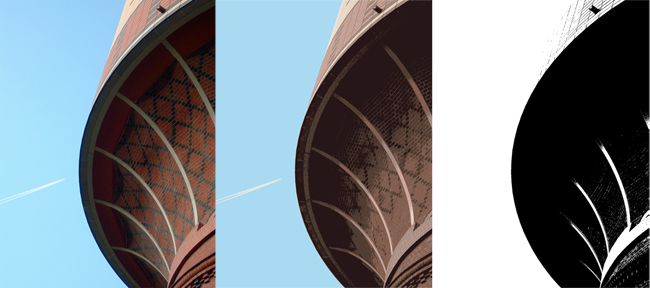
\includegraphics[width=.9\linewidth]{./farbanzahl.jpg}
\end{center}
\subsubsection{Farbmodelle}
\label{sec:orgb42a74c}
\textbf{Graustufen}: Das Bild wird auf Graustufen reduziert. So können Sie Farbaufnahmen nachträglich in schwarzweiß-Bilder konvertieren. Bei einer 8-Bit Kodierung stehen 256 Graustufen zur Verfügung.

\textbf{Indizierte Farben}: Das Bild wird in maximal 256 Farben konvertiert. Wenn das Ausgangsbild ein Farbbild ist, dann erscheint ein Popup-Fenster Indizierte Farben. Hier können Sie bestimmen, wie viele Farben verwendet werden dürfen. Photoshop generiert automatisch eine Farbtabelle zu dem Bild, die beim Speichern der Datei beigefügt wird.

\textbf{RGB Farbe}: Hierbei handelt es sich um das klassische Farbmodell für Bildschirmdarstellungen. Es eignet sich für lichtemitierende Medien wie Bildschirme oder auch Beamer. Die Farbwerte des Bildes werden in Rot-, Grün- und Blauanteile aufgespalten und einzeln kodiert. Die Mischung der Farben erfolgt additiv, d.h. wenn alle drei Farbkomponenten in voller Ausprägung vorhanden sind erscheint das Ergebnis weiß. Der Farbraum des RGB-Modells ist ein Würfel mit Einheitskantenlänge (von 0 bis 1) wie er folgend abgebildet ist. Die Einheitsvektoren sind die Farben Rot, Grün und Blau. Im Ursprung liegt Schwarz, die Grauwerte liegen auf der Hauptdiagonalen.
\url{./farbmodell.gif}

\textbf{CMYK-Farbe}: Die im CMY-Farbraum verwendeten Farben Cyan, Magenta und Gelb (Yellow) stehen komplementär zu den Komponenten des RGB-Farbraumes. Entsprechend verhalten sie sich auch komplementär: Mischt man alle drei Farben, so erhält man Schwarz. Das Farbmodell ist also subtraktiv. Man spricht auch von Körperfarben, da sich die Komponenten ähnlich der körperhaften Farben eines Malkastens mischen. Das Modell wird im Druck verwendet.
Auch das CMY-Farbmodell ist ein Würfel folgend gezeigt. In der Praxis hat sich das CMY-Farbmodell als unzureichend erwiesen. Die Mischung aller drei Komponenten führt nur theoretisch zu einem klaren Schwarz, praktisch aber zu einem sehr dunklen Braunton. Die Qualität wird dadurch erhöht, dass tatsächlich zusätzlich Schwarz beigemischt wird. Man spricht dann vom CMYK-Farbmodell, wobei K für Key-Color (i.e. Schwarz) steht.
\url{./farbmodell2.gif}
Ein zusätzlicher Vorteil entsteht dadurch, dass sämtliche Farben durch die Beimischung von Schwarz verdunkelt werden können, also insgesamt deutlich weniger an Farbe auf das Papier aufgetragen werden muss.
\subsection{Bildgröße}
\label{sec:orgf50c9fc}
Anzahl der Pixel und Farbtiefe sind die ausschlaggebenden Variablen für die Menge der entstehenden Daten. Sie werden als Bildgröße bezeichnet.\\
Mit Bildgröße wird in der Digitaltechnik nicht die räumliche Größe eines Bildes bezeichnet, sondern die Menge der Daten, die zu seiner Beschreibung verwendet werden. Diese hängen zum einen von der Anzahl der Pixel und zum anderen von der Farbtiefe ab. Die Größe der Datei wird dabei wie folgt berechnet:
\(G = M * N * Fb\) wobei G = Bildgröße, M \& N = räumliche Ausdehnung und Fb = Farbtiefe in Byte

Ein Bild der Aufloesung von 1024x768 und einer RGB-Farbtiefe von 24 Bit benötigt beispielsweise 2.36MB Speicherplatz: \(G = 1024 * 768 * (24/3) = 2.36\)

Die Anzahl der Pixel sagt noch nichts über die räumliche Größe eines Bildes aus, denn die physische Ausdehnung eines Pixels ist nicht standardisiert. Sie muss festgelegt werden. Diese Festlegung erfolgt über den Begriff der Auflösung, die in ppi (pixel per inch) angegeben wird. Hier wird festgelegt, wieviele Pixel auf einem Inch, bzw. Zoll (ca. 2,54 cm) verteilt sind. Da bei Fotografien Pixel in der Regel eine quadratische Form haben, reicht hier eine einzelne Angabe. Es ist aber durchaus möglich in der Horizontalen eine andere Länge als in der Vertikalen anzugeben.\\
Für reine Bildschirmdarstellungen reichen bereits 72 ppi aus. Damit werden auf einem Quadratzoll des Monitors 722 Pixel dargestellt. Das entspricht der Auflösung handelsüblicher Monitore, eine höhere Auflösung macht hier also keinen Sinn. Anders sieht es im Druck aus. Hier werden 300 bis 600 Punkte als Minimum angesehen, um zu verhindern, dass das Bild gerastert erscheint.\\
Beispiel: Ein Bild mit der physischen Ausdehnung 10x15 cm (ca. 3,937 Zoll x 5,91 Zoll) und einer RGB-Farbtiefe von 24 Bit hat eine Auflösung von 300 ppi. Der Speicherbedarf berechnet sich wie folgt:
\begin{itemize}
\item geg: M = 10cm = 3,937 Zoll; N = 15cm = 5,91 Zoll, Fb =  24 Bit, Auflösung A = 300ppi
\end{itemize}
\begin{itemize}
\item ges: G
\end{itemize}
\begin{equation}
\begin{split}
G = (M*A) * (N*A) * Fb\\
  = (3,937 * 300) * (5,91 * 300) * (24/8)\\
  = 1.181 * 1.773 * 3\\
  = 6.281.739 \text{Byte} = 6.1 \text{MB}
\end{split}
\end{equation}
\subsection{Dateiformate}
\label{sec:org6509309}
Die Größe einer Bilddatei hängt zum einen von der physischen Bildgröße ab, zum anderen aber auch von den Methoden, die bei der Speicherung verwendet werden. Diese hängen wiederum davon ab, was und mit welchem Kompressionsverfahren gespeichert werden soll.\\
Welche Größe Bilddateien erreichen und welches Dateiformat verwendet werden sollte, hängt von verschiedenen Faktoren ab. Eine der wichtigsten Grundfragen ist beispielsweise, ob die in Photoshop verwendeten Ebenen tatsächlich auch als Ebenen abgespeichert werden sollen. Der Vorteil liegt darin, dass zu einem späteren Zeitpunkt oder sogar auch mit einem anderen Programm an dem Bild auf Basis der Ebenen weitergearbeitet werden kann. Reduziert man jedoch alle Ebenen auf nur eine Ebene oder wählt ein Dateiformat, dass die Speicherung verschiedener Ebenen nicht zulässt, dann können diese auch durch erneutes Öffnen der Datei nicht wieder hergestellt werden. Der Nachteil liegt ganz klar in einer deutlich größeren Datei.
\end{document}
